\section*{Unit 2}

\setcounter{section}{2}
\setcounter{subsection}{0}

\subsection{The idea of limit --- (Non-rigorous) examples}

\underline{Example 1}:

\(\DS f(x) = \frac{x^{2} - 1}{x - 1}\)

\(f(1)\) is undefined.

We can simplify \(f\) as follows.

\[\frac{x^{2} - 1}{x - 1} = \frac{\br{x - 1} \br{x + 1}}{x - 1} = x + 1 \quad \fbox{\text{if} x \neq 1}\]

This means that \(f\) is just a line, but the point at \(x = 1\) is missing.

If we look at all of the values near \(f(1)\), we can see that they go toward \(2\). This is the informal idea of limit. The notation for this is \(\DS \lim_{x \to 1} f(x) = 2\) which is read as ``The limit as \(x\) approaches \(1\) of \(f(x)\) is \(2\).''

If \(x\) is very close to \(1\) (but \(x \neq 1\)), then \(f(x)\) is very close to \(2\).

\underline{Example 2}:

\(\DS f(x) = \frac{1 - \sqrt{1 + x}}{x}\).

Domain \(f = [-1, 0) \cup (0, \infty)\).

\(f(0)\) is undefined.

\begin{tabular}{c|c}
  \(x\) & \(f(x)\) \\
  \midrule
  1 & -0.4142135625 \\
  0.1 & -0.4880884817 \\
  0.01 & -0.4987562112 \\
  0.001 & -0.4996750625 \\
\end{tabular}

As \(x\) gets very close to \(0\), \(f(x)\) gets very close to \(-0.5\). If \(x\) is very close to \(0\) (but \(x \neq 0\)), then \(f(x)\) is very close to \(-0.5\).

Another way to understand this is some simplification. We can take \(f(x)\) and multiply and divide by the conjugate of the numerator.

\[\frac{1 - \sqrt{1 + x}}{x} = \frac{\br{1 - \sqrt{1 + x}} \br{1 + \sqrt{1 + x}}}{x \br{1 + \sqrt{1 + x}}} = \cdots = \frac{-1}{1 + \sqrt{1 + x}} \quad \fbox{\text{when} x \neq 0}\]

The new function has a vaule of \(-0.5\) at \(x = 0\). So even when \(f(0)\) is not defined, we can draw a conclusion as to what it is likely to be.

\underline{Summary}:

\(\DS \lim_{x \to a} f(x) = L\) roughly means that ``If \(x\) is close to \(a\) (but \(x \neq a\)), then \(f(x)\) is close to \(L\).''

\subsection{Examples of limits that do not exist}

\underline{Example 1}:

\(h(x) = \sin{\frac{\pi}{2x}}\)

\(h(0)\) is undefined

\begin{tabular}{c|c}
  \(x\) & \(f(x)\) \\
  \midrule
  1 & 1     \\
  1/2 & 0   \\
  1/3 & -1  \\
  1/4 & 0   \\
  1/5 & 1   \\
  1/6 & 0   \\
  1/7 & -1  \\
  1/8 & 0   \\
\end{tabular}

% TODO add graph

The function oscilates infinitely many times before reaching 0, so it never reaches 0. Similar to Achilles and the turtle (Zeno's paradox).

If \(x\) is close to \(0\), then \(h(x)\) is not close to one number.

We say that \(\DS \lim_{x \to 0} h(x) DNE\).

\underline{Example 4}:

\(F(x) = \frac{1}{\br{x - 1}^{2}}\).

\(F(1)\) is undefined.

This function has a vertical asymptote at \(x = 1\).

If \(x\) is close to \(1\) (but \(x \neq 1\)), then \(F(x)\) is very large.

We describe this case with the notation \(\DS \lim_{x \to 1} F(x) = \infty\). This also means, however, that the limit does not exist. The limit does not exist because for the limit to exist, \(F(x)\) must approach one single number but it is not approaching a single number as it is increasing to infinity.

% TODO add graph

\subsection{Side limits}

\underline{Example 1}:

\(\DS G(x) = \frac{x^{2} + x}{\abs{x}}\).

\(G(0)\) is undefined.

Since we are dealing with an absolute value here, we will break it into two cases.

If \(x > 0\), then \(\abs{x} = x\). This means that in this case, \(G(x) = \frac{x \br{x + 1}}{x} = x + 1\).

If \(x < 0\), then \(\abs{x} = -x\). This means that in this case, \(G(x) = \frac{x \br {x - 1}}{-x} = -x - 1\).

% TODO add graph

When \(x\) is close to \(0\), \(G(x)\) is not close to one single number, but instead two numbers. This means that \(\DS \lim_{x \to 0} G(x) \text{DNE}\).

We describe this case as a ``Side Limit.'' We say that \(\DS \lim_{x \to 0^{+}} G(x) = 1\) and that \(\DS \lim_{x \to 0^{-}} G(x) = -1\). The superscript denotes the side of the limit that we are approaching from.

\subsection{Distance and absolute values}

The best way to describe absolute value algebraicly is to break it into two cases.

For every \(x \in \R, \abs{x} = \begin{cases} x \quad & \text{if } x \geq 0 \\ -x \quad & \text{if } x < 0 \end{cases}\).

The best way to describe absolute value geometrically is as follows.

\begin{itemize}
  \item \(\abs{x}\) is the distance between \(x\) and \(0\).
  \item \(\abs{x - a}\) is the distance between \(x\) and \(a\).
\end{itemize}

Some properties of absolute values:

For every \(x, y \in \R\),

\begin{itemize}
  \item \(\abs{xy} = \abs{x} \abs{y}\)
  \item \(\abs{x + y} \leq \abs{x} + \abs{y}\)
\end{itemize}

\underline{Equivalent expressions: \(\abs{x - a} < \delta\)}:

\fbox{\color{red}The distance between \(x\) and \(a\) is smaller than \(\delta\)}

\begin{itemize}
  \item \(\abs{x - a} < \delta\)
  \item \(- \delta < x - a < \delta\)
  \item \(a - \delta < x < a + \delta\)
\end{itemize}

Any time you see one of these inequalities, you can move back and forth between these terms.

\subsection{The formal definition of limit}

We have the rough idea:
\[\lim_{x \to a} f(x) = L\]
If \(x\) is close to \(a\) (but \(x \neq a\)), then \(f(x)\) is close to \(L\).

\begin{itemize}
  \item ``\(x\) is close to \(a\)''

        \(\abs{x - a}\) is ``small'', \quad \(\abs{x - a} < \delta\)

  \item ``\(x\) is close to \(a\) (but \(x \neq a\))''

        \(0 < \abs{x - a} < \delta\)

  \item ``If \(x\) is close to \(a\) (but \(x \neq a\)), then \(f(x)\) is close to \(L\)''

        \(0 < \abs{x - a} < \delta \implies \abs{f(x) - L} < \varepsilon\)
\end{itemize}

\begin{mdframed}

  \underline{Definition of Limit}

  Let \(a, L \in \R\). Let \(f\) be a function defined, at least, on an interval centered at \(a\), excapt maybe at \(a\).

  We say that \(\DS \lim_{x \to a} f(x) = L\) when \(\forall \varepsilon > 0, \exists \delta > 0 \st 0 < \abs{x - a} < \delta \implies \abs{f(x) - L} < \varepsilon\).

\end{mdframed}

\subsection{Limits at infinity}

\(\DS f(x) = \frac{x + 1}{x} = 1 + \frac{1}{x}\)

As \(\DS x \to \infty, \frac{1}{x} \approx 0, f(x) = 1 + \frac{1}{x} \approx 1\).

\(\DS \lim_{x \to \infty} f(x) = 1\)

% TODO add graph y = f(x) and y = L where f(x) = x + 1 / x and L = 1

\(\lim_{x \to \infty} f(x) = L\)

To describe this with inequalities, we can convert the concepts as follows.
\begin{align*}
x \text{ large } &\implies f(x) \text{ close to } L \\
x > {\color{red}M} &\implies \abs{f(x) - L} < {\color{red}\varepsilon}
\end{align*}

We can write this more formally, quantifying the variables \(M\) and \(\varepsilon\) as

\begin{mdframed}
  \underline{Definition of Limit at Infinity}

  Let \(L \in \R\). Let \(f\) be a function defined, at least, on an interval of the form \((p, \infty)\) for some \(p \in \R\).

  We say that \(\DS \lim_{x \to \infty} f(x) = L\) when:

  \[\forall \varepsilon > 0, \exists M \in \R \st x > M \implies \abs{f(x) - L} < \varepsilon\]
\end{mdframed}

\subsection{Prove a function has a limit from the definition --- Example 1}

Prove directly from the formal definiton of limit that \(\DS \lim_{x \to 3} (2x + 1) = 7\)

We want to show:
\[\forall \varepsilon > 0, \exists \delta > 0 \st 0 < \abs{x - 3} < \delta \implies \abs{\br{2x + 1} - 7} < \varepsilon\]

\begin{enumerate}
  \item Let \(\varepsilon > 0\)
  \item Take \(\delta = \)? \(\delta\) can be a function of \(\varepsilon\).
  \item Let \(x \in \R\), assume \(0 < \abs{x - 3} < \delta\)
  \item Prove that \(\abs{\br{2x + 1} - 7} < \varepsilon\)
\end{enumerate}

\begin{proof} \(\)

  Let \(\varepsilon > 0\). Take \(\delta = \frac{\varepsilon}{2}\). Let \(x \in \R\).

  Assume that \(0 < \abs{x - 3} < \delta\).

  Then
  \[\abs{\br{2x + 1} - 7} = \abs{2x + 6} = 2 \abs{x - 3} < 2 \delta = \varepsilon\]
  And thus I have proven that \(\abs{\br{2x + 1} - 7} < \varepsilon\), as needed. \qedhere
\end{proof}

\subsection{Prove a function has a limit from the definition --- Example 2}

Prove directly from the definition of limit, that \(\DS \lim_{x \to 4} \br{x^{2} + 1} = 17\).

WTS \(\forall \varepsilon > 0, \exists \delta > 0 \st 0 < \abs{x - 4} < \delta \implies \abs{\br{x^{2} + 1} - 17} < \varepsilon\).

\underline{Rough Work}:
\begin{align*}
  &\abs{\br{x^{2} + 1} - 17} \\
  =&\abs{x^{2} - 16} \\
  =&\abs{\br{x + 4} \br{x - 4}} \\
  =&\abs{x + 4} \abs{x - 4} \\
  <&\abs{x + 4} \cdot \delta
\end{align*}
We are not allowed to take \(\delta\) based on \(x\). Taking \(\delta = \frac{\varepsilon}{\abs{x + 4}}\) is a bad idea.

If we can make \(\abs{x + 4} < C\) for some number \(C\), then and \(\delta < \frac{\varepsilon}{C}\) will work.

If we choose \(\delta \leq 1\), then \(\abs{x + 4} < 1 \implies 3 < x < 5 \implies 7 < x + 4 < 9 \implies \abs{x + 4} < 9\)

So I need \(\delta \leq 1 \tand \delta \leq \frac{3}{9}\) at the same time. {\color{red}Take \(\delta = \min\cbr{1, \frac{\varepsilon}{9}}\)}

\begin{proof} \(\)

  Let \(\varepsilon > 0\). Take \(\delta = \min\cbr{1, \frac{\varepsilon}{9}}\). Let \(x \in \R\).

  Assume \(0 < \abs{x - 4} < \delta\). This implies
  \begin{itemize}
    \item \(\abs{x - 4} < \frac{\varepsilon}{9}\)
    \item \(\abs{x - 4} < 1\). Hence \(3 < x < 5\), and \(7 < x + 4 < 9\).
  \end{itemize}

  Thus: \(\DS \abs{\br{x^{2} + 1} - 17} = \abs{x^{2} - 16} = \abs{x - 4} \abs{x + 4} < \frac{\varepsilon}{9} \cdot 9 = \varepsilon\).

  We have proven \(\abs{\br{x^{2} + 1} - 17} < \varepsilon\), as needed. \qedhere
\end{proof}

\subsection{How to prove a limit DNE from the definition}

Let \(h(x) = \cos\br{\pi x}\). Prove, from the definition of limit that \(\DS \lim_{x \to \infty} h(x)\) does not exist.

% TODO add graph

\(\lim_{x \to \infty} h(x) = L\) means: \(\forall \varepsilon > 0, \exists M \in \R \st \br{\forall x \in \R,} x > M \implies \abs{h(x) - L} < \varepsilon\).

\(\lim_{x \to \infty} h(x) \neq L\) means: \(\exists \varepsilon > 0\st \forall M \in \R, \exists x \in \R \st x > M \tand \abs{h(x) - L} < \varepsilon\).

\(\lim_{x \to \infty} h(x) \dne\) means: \(\forall L \in \R, \exists \varepsilon > 0 \st \forall M \in \R, \exists x \in \R \st x > M \tand \abs{h(x) - L} \geq \varepsilon\).

We want to show that \(\DS \lim_{x \to \infty} h(x) \dne\). This means we want to show \[\forall L \in \R, \exists \varepsilon > 0 \st \forall M \in \R, \exists x \in \R \st x > M \tand \abs{h(x) - L} \geq \varepsilon\]

\underline{Structure}
\begin{enumerate}
  \item Let \(L \in \R\)
  \item Take \(\varepsilon =~???\)
  \item Let \(M \in \R\)
  \item Take \(x =~???\)
        \item Verify that \(x > M\), and \(\abs{h(x) - L} \geq \varepsilon\)
\end{enumerate}

% TODO add graph from https://youtu.be/VOEzUbNTCSk?t=383

Pick \(\varepsilon \geq 1\). Then \(1\) or \(-1\) \(\notin (L - \varepsilon, L + \varepsilon)\)

Pick \(x \in \Z\). Then \(h(x) = 1 \tor -1\)

\begin{proof} \(\)

  Let \(L \in \R\). Take \(\varepsilon = \frac{1}{2}\). Let \(M \in \R\).

  At least one of the following must be true:

  \begin{itemize}
    \item Case A:\quad \(1 \notin (L - \varepsilon, L + \varepsilon)\)

          I choose any \(x \in \Z\), even, satisfying \(x > M\).

          Then \(h(x) = 1\)

    \item Case B:\quad \(-1 \notin (L - \varepsilon, L + \varepsilon)\)

          I choose any \(x \in \Z\), odd, satisfying \(x > M\).

          Then \(h(x) = - 1\)
  \end{itemize}
  Either way, it satisfies \(x > M\) and \(\abs{h(x) - L} \geq \varepsilon\), as needed. \qedhere
\end{proof}

\subsection{Limit laws}

I want to prove rigorously that, for every polynomial \(P\) and every \(a \in \R\):
\[\lim_{x \to a} P(x) = P(a)\]

To do this, we need to prove some basic limit that can be used to construct all other limits of polynomials.
\[\lim_{x \to a} x = a \tand \lim_{x \to a} c = c\]

Then we must prove the Limit Laws

Assume \(\DS \lim_{x \to a} f(x) = L\) and \(\DS \lim_{x \to a} g(x) = M\).

Then:
\begin{itemize}
  \item \(\DS \lim_{x \to a} \sbr{f(x) + g(x)} = L + M\)
  \item \(\DS \lim_{x \to a} \sbr{f(x) \cdot g(x)} = L \cdot M\)
  \item \(\DS \lim_{x \to a} \sbr{\frac{f(x)}{g(x)}} = \frac{L}{M} \quad (\text{assuming } M \neq 0)\)
\end{itemize}

Then, we can use these. For example, prove that \(\DS \lim_{x \to 2} \br{x^{4} - 3x} = 10\)

\begin{proof} \(\)
  \begin{align*}
    &~\lim_{x \to 2} \br{x^{4} - 3x} \\
    =&~\br{\lim_{x \to 2} x^{4}} + \br{\lim_{x \to 2} -3x} && \text{(Limit Law for sum)} \\
    =&~\br{\lim_{x \to 2} x}^{4} + \br{\lim_{x \to 2} -3} \br{\lim_{x \to 2} x} && \text{(Limit Law for product)}  \\
    =&~\br{2}^{4} + \br{-3} \br{2} && \text{(Basic Limits)} \\
    =&~10
  \end{align*}
\end{proof}

The same process will work for every polynomial! One thing to note is that the limit laws only apply if the initial limit exists.

\subsection{Proof of the limit law for sums}

\begin{mdframed}
  \underline{Theorem}

  Let \(a, L, M \in \R\). Let \(f\) and \(g\) be functions defined at least on an interval cenetered at \(a\), except maybe at \(a\).

  IF \(\DS \lim_{x \to a} f(x) = L\) and \(\DS \lim_{x \to a} g(x) = M\) THEN \(\DS \lim_{x \to a} \sbr{f(x) + g(x)} = L + M\)
\end{mdframed}

Call \(h = f + g\).

WTS \(\forall \varepsilon > 0, \exists \delta > 0 \st 0 < \abs{x - a} < \delta \implies \abs{h(x) - {L + M}} < \varepsilon\).

We need \(0 < \abs{x - a} < \delta \implies \abs{h(x) - {L + M}} < \varepsilon\)
\[\abs{h(x) - \br{L + M}} \leq \abs{f(x) - L} + \abs{g(x) - M}\]
Make \(\DS \abs{f(x) - L} < \frac{\varepsilon}{2}\). We can do this because we \emph{know} \(\DS \lim_{x \to a} f(x) = L\).

For the value \(\DS \frac{\varepsilon}{2}, \exists \delta_{1} > 0 \st 0 < \abs{x - a} < \delta_{1} \implies \abs{f(x) - L} < \frac{\varepsilon}{2}\).

We can do the same thing for \(g\) resulting in the number \(\delta_{2}\).

Thus we have concluded that:
\[\exists \delta_{1} > 0 \st 0 < \abs{x - a} < \delta_{1} \implies \abs{f(x) - L} < \frac{\varepsilon}{2}\]
\[\exists \delta_{2} > 0 \st 0 < \abs{x - a} < \delta_{2} \implies \abs{g(x) - M} < \frac{\varepsilon}{2}\]
Take \(\delta = \min\cbr{\delta_{1}, \delta_{2}}\).

\begin{proof} \(\)

  Let \(\varepsilon > 0\).

  I use \(\frac{\varepsilon}{2}\) in the definition of \(\DS \lim_{x \to a} f(x) = L\). \[\exists \delta_{1} > 0 \st 0 < \abs{x - a} < \delta_{1} \implies \abs{f(x) - L} < \frac{\varepsilon}{2}\]

  I use \(\frac{\varepsilon}{2}\) in the definition of \(\DS \lim_{x \to a} g(x) = M\). \[\exists \delta_{2} > 0 \st 0 < \abs{x - a} < \delta_{2} \implies \abs{g(x) - M} < \frac{\varepsilon}{2}\]

  Take \(\delta = \min\cbr{\delta_{1}, \delta_{2}}\).

  Let \(x \in \R\). Assume \(0 < \abs{x - a} < \delta\). This implies:
  \begin{itemize}
    \item \(0 < \abs{x - a} < \delta_{1}\). Thus \(\abs{f(x) - L} < \varepsilon/2\)
    \item \(0 < \abs{x - a} < \delta_{2}\). Thus \(\abs{g(x) - M} < \varepsilon/2\)
  \end{itemize}

  Then \(\abs{h(x) - \br{L + M}} = \abs{\sbr{f(x) - L} + \sbr{g(x) - M}} \leq \abs{f(x) - L} + \abs{g(x) - M} < \frac{\varepsilon}{2} + \frac{\varepsilon}{2} = \varepsilon\)

  And thus we have shown that \(\abs{h(x) - \br{L + M}} < \varepsilon\), as needed. \qedhere
\end{proof}

\subsection{The Squeeze Theorem}

\underline{Exercise}

Compute \(\DS \lim_{x \to 0} x^{2} \sin \frac{1}{x}\).

\underline{An {\color{red}Incorrect} Solution}

\[\lim_{x \to 0} \sbr{x^{2} \sin \frac{1}{x}} = \sbr{\lim_{x \to 0} x^{2}} \cdot \sbr{\lim_{x \to 0} \sin \frac{1}{x}} = 0 \cdot \sbr{\lim_{x \to 0} \sin \frac{1}{x}} = 0\]

This is incorrect as we can only use limit laws when the limits exist. In this calculation, we have used the limit law for products. The function \(\sin \frac{1}{x}\) does not have a limit at \(0\) as it oscilates infinitely near \(0\).

\underline{Correct Solution}

For every \(x \neq 0\):

\begin{align*}
-1 &\leq \sin \frac{1}{x} \leq 1 \\
-x^{2} &\leq x^{2} \sin \frac{1}{x} \leq x^{2} \\
-x^{2} &\leq x^{2} \sin \frac{1}{x} \leq x^{2} \\
\end{align*}

% TODO add graph y = x^2, y = - x^2, y = x^2 sin 1/x
\begin{center}
  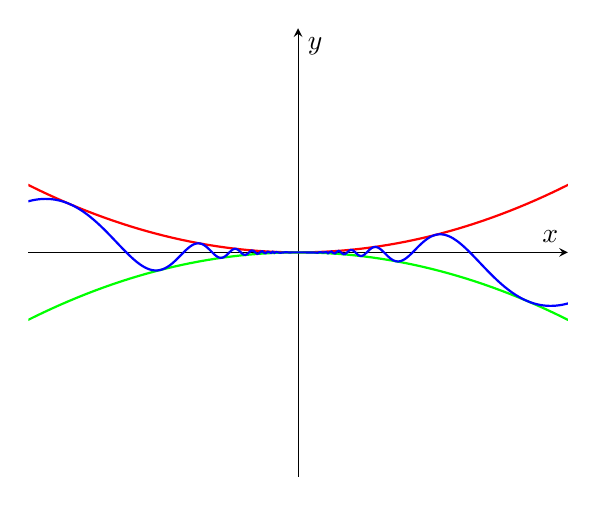
\begin{tikzpicture}
    \begin{axis}[
      ticks=none,
      axis lines=middle,
      axis equal,
      xlabel=\(x\),
      ylabel=\(y\),
      xmin=-0.25,
      xmax=0.25,
      ymin=-0.125,
      ymax=0.125,
      yticklabels={,,},
      xticklabels={,,}
      ]
      % \draw[dashed,thick,color=red] (axis cs: 1, 1.5) -- (axis cs: 1, 0) node[below] (endofplotsquare) {\(x_{1}\)};
      \addplot [
      thick,
      color=red,
      domain=-4:4,
      samples=1000
      ]
      {x^2};
      \addplot [
      thick,
      color=green,
      domain=-4:4,
      samples=1000
      ]
      {-x^2};
      \addplot [
      thick,
      color=blue,
      domain=-4:4,
      samples=5000
      ]
      {x^2 * sin(deg(1/(x)))};
    \end{axis}
  \end{tikzpicture}
\end{center}

\begin{mdframed}
  \underline{The Squeeze Theorem}

  Let \(a, L \in \R\). Let \(f, g, \tand h\) be functions defined near \(a\), except possibly at \(a\).

  If
  \begin{itemize}
    \item \(\DS \exists p > 0 \st 0 < \abs{x - a} < p \implies h(x) \leq g(x) \leq f(x)\)
    \item \(\DS \lim_{x \to a} f(x) = L\)
    \item \(\DS \lim_{x \to a} h(x) = L\)
  \end{itemize}
  Then \(\DS \lim_{x \to a} g(x) = L\)
\end{mdframed}

Since we know that for every \(x \neq 0,~x^{2} \sin \frac{1}{x}\) is ``squeezed'' by \(-x^{2} \tand x^{2}\), we know that \(\DS \lim_{x \to 0} -x^{2} = \lim_{x \to 0} x^{2} = \lim_{x \to 0} \sbr{x^{2} \sin \frac{1}{x}} = 0\).

\subsection{Proof of the Squeeze Theorem}

WTS \(\forall \varepsilon, \exists \delta > 0 \st 0 < \abs{x - a} < \delta \implies \abs{g(x) - L} < \varepsilon\)

\underline{Rough Work}

\(\abs{g(x) - L} < \varepsilon\) is equivalent to \(L - \varepsilon < g(x) < L + \varepsilon\).

We \emph{know} \(0 < \abs{x - a} < p \implies h(x) \leq g(x) \leq f(x)\).

We \emph{know} \(\DS \lim_{x \to a} f(x) = L\). \[\exists \delta_{1} > 0 \st 0 < \abs{x - a} < \delta_{1} \implies L - \varepsilon < f(x) < L + \varepsilon\]

We \emph{know} \(\DS \lim_{x \to a} h(x) = L\). \[\exists \delta_{2} > 0 \st 0 < \abs{x - a} < \delta_{2} \implies L - \varepsilon < h(x) < L + \varepsilon\]

If we combine the inequalities that we know, \(h(x) \leq g(x) \leq f(x)\),  \(f(x) < L + \varepsilon\), \(L - \varepsilon < h(x)\), we can conclude what we need.

Take \(\delta = \min\cbr{\delta_{1}, \delta_{2}, p}\).

\begin{proof} \(\)

  Let \(\varepsilon > 0\).

  Use same \(\varepsilon\) in the definition of \(\DS \lim_{x \to a} f(x) = L\). \(\DS \exists \delta_{1} > 0 \st 0 < \abs{x - a} < \delta_{1} \implies \abs{f(x) - L} < \varepsilon \implies f(x) < L + \varepsilon\)

  Use same \(\varepsilon\) in the definition of \(\DS \lim_{x \to a} h(x) = L\). \(\DS \exists \delta_{2} > 0 \st 0 < \abs{x - a} < \delta_{2} \implies \abs{h(x) - L} < \varepsilon \implies L - \varepsilon < h(x)\)

  Take \(\delta = \min\cbr{\delta_{1}, \delta_{2}, p}\).

  Let \(x \in \R\). Assume \(0 < \abs{x - a} < \delta\). This implies:
  \begin{itemize}
    \item \makebox[4cm][l]{\(0 < \abs{x - a} < \delta_{2}\)} Thus \(L - \varepsilon < h(x)\)
    \item \makebox[4cm][l]{\(0 < \abs{x - a} < p\)} Thus \(h(x) \leq g(x) \leq f(x)\)
    \item \makebox[4cm][l]{\(0 < \abs{x - a} < \delta_{1}\)} Thus \(f(x) < L + \varepsilon\)
  \end{itemize}

  Therefore \(L - \varepsilon < g(x) < L + \varepsilon\). Equivalently, we have proven that \(\abs{g(x) - L} < \varepsilon\), as needed. \qedhere
\end{proof}

\subsection{The definition of continuity}

``A function is continuous when its graph can be drawn without lifting the pen from the paper.''

\begin{mdframed}

  \underline{Definition of Continuity}

  Let \(a \in \R\). Let \(f\) be a function defined, at least, on an interval centered at \(a\).

  We say that \(f\) is continuous when \(\DS \lim_{x \to a} f(x) = f(a)\).
\end{mdframed}

This means:
\begin{enumerate}
  \item The limit exists
  \item \(f(a)\) is defined
  \item \(\DS \lim_{x \to a} f(x) = f(a)\)
\end{enumerate}

\begin{mdframed}

  \underline{An equivalent definition (Epsilon Delta Definition of Continuity)}

  Let \(a \in \R\). Let \(f\) be a function defined, at least, on an interval centered at \(a\).

  We say that \(f\) is continuous at \(a\) when

  \[\forall \varepsilon > 0, \exists \delta \st \abs{x - a} < \delta \implies \abs{f(x) - f(a)} < \varepsilon\]

\end{mdframed}

Continuous at a point: \(f\) continuous at \(c\) means \(\DS \lim_{x \to c} f(x) = f(c)\)

Continuous on an open interval: \(f\) continuous on the interval \((a, b)\) means \(\forall c \in (a, b),~f\) is continuous at \(c\)

Continuous on a closed interval: \(f\) continuous on the interval \([a, b]\) means
\begin{enumerate}
  \item \(\DS \lim_{x \to a^{+}} f(x) = f(a)\)
  \item \(\forall c \in (a, b),~f\) is continuous at \(c\)
  \item \(\DS \lim_{x \to b^{-}} f(x) = f(b)\)
\end{enumerate}

\subsection{The main continuity theorem}

\begin{mdframed}

  \underline{The Main Continuity Theorem}

  Any function we can construct with sum, product, quotient, and composition of polynomials, roots, trigonometric functions, exponentials, logarithms, and absolute values is continuous (on its domain).
\end{mdframed}

Example: \[\lim_{x \to 1} \frac{x^{2} - \sin x}{e^{x} + \ln\br{\sqrt{x} + 3}} = \frac{1 - \sin 1}{e + \ln 4}\]

\subsection{Limits and composition of functions}

We do not have a ``Limit Law'' for compositions. Just knowing that two functions have limits does not guarantee that the composition of the two functions has a limit.

\underline{False Theorem}

If \(\DS \lim_{x \to a} f(x) = L \tand \lim_{y \to L} g(y) = M\)

\(\cancel{\text{Then \(\DS \lim_{x \to a} g(f(x)) = M?\)}}\)

\begin{mdframed}

  \underline{Theorem 1}

  If \(f\) continuous at \(a\), and \(g\) continuous at \(f(a)\)

  Then \(g \circ f\) continuous at \(a\).

\end{mdframed}

% A counter example for the false theorem is as follows.

% \(f(x) = \begin{cases} x \sin \frac{\pi}{x} & \text{ if } x \neq 0 \\ 0 & \text{ if } x = 0 \end{cases}\)

% \(g(y) = \begin{cases} 2 & \text{ if } y = 0 \\ 1 & \text{ if } y \neq 0 \end{cases}\)

% \(g(f(x)) = \begin{cases} 2 & \text{ if } x \dots \\ 1 & \text{ if } x \dots \end{cases}\)

To get to the core of the probelm, we can look at what the theorems are really saying.

\begin{itemize}
  \item \(\DS \lim_{x \to a} f(x) = L\) means:

        \(\cbr{x \text{ close to } a, x \neq a} \implies f(x) \text{ close to } L\).

  \item \(f\) continuous at \(a\) means:

        \(x \text{ close to } a \implies f(x) \text{ close to } f(a)\).
\end{itemize}

Let us look at \emph{Theorem 1}.

The first hypothesis means \(x \text{ close to } a \implies f(x) \text{ close to } f(a)\).

The second hypothesis means \(y \text{ close to } f(a) \implies g(y) \text{ close to } g(f(a))\).

We can concatenate the two implications to form \(x \text{ close to } a \implies g(f(x)) \text{ close to } g(f(a))\).

By contrast, let us try and do the same thing with the \emph{False Theorem}.

The first hypothesis means \(x \text{ close to } a \text{ but } x \neq a \implies f(x) \text{ close to } L\).

The second hypothesis means \(y \text{ close to } L \text{ but } y \neq L \implies g(y) \text{ close to } M\).

We cannot concatenate these two implications as the ``then'' part in the first does not match the ``if'' part in the second. This is why the theorem is false.

But we can fix the theorem!

\begin{mdframed}
  \underline{Theorem 2}

  If
  \begin{itemize}
    \item \(\DS \lim_{x \to a} f(x) = L\)
    \item \(\DS f(x) \neq L\) for \(x\) on an interval centered at \(a\), excepy maybe at \(a\).
    \item \(\DS \lim_{y \to L} g(y) = M\)
  \end{itemize}

  Then \(\DS \lim_{x \to a} g(f(x)) = M\)
\end{mdframed}

\begin{mdframed}
  \underline{Theorem 3}

  If
  \begin{itemize}
    \item \(\DS \lim_{x \to a} f(x) = L\)
    \item \(g\) is continuous at \(L\)
  \end{itemize}

  Then \(\DS \lim_{x \to a} g(f(x)) = g(L)\)
\end{mdframed}

\subsection{Discontinuties (and how to remove them)}
\subsection{A geometric proof for a trigonometric limit}
\subsection{Review of basic techniques for computing limits}
\subsection{How to compute the limit of a rational function at infinity}
\subsection{The Extreme Value Theorem}
\subsection{The Intermediate Value Theorem}
